\subsection{Vulnerable Fuel Dispensers}
\label{sec:bkgd-vuln}

xxx \note{END OF KL EDITS} xxx

hysical security of fuel dispensers 

Unfortunately, circumventing current physical security measures has not posed a challenge to criminals~\cite{ny-fuel-paymentdoor-access}.
%
Fuel dispensers include physical security protections, including keyed access,
and tamper-evident seals, however we explain how both can be easily defeated.
%
One of the primary reasons why physical security on fuel pumps is weak is that
many people need access to the pumps, including fuel station employees,
government inspectors, and service technicians.

xxx \note{END OF KL EDITS} xxx

In this section we provide an overview of how criminals can exfiltrate payment
information with a skimmer residing entirely inside a PoS terminal.
%
First, we describe the components of internal skimmers, and how they can
be constructed with commodity hardware.
%
Then, we explain how criminals exploit vulnerabilities in fuel dispenser design
to quickly install internal skimmers.

\subsection{Design of Internal Skimmers} %{{{
\label{sec:background:design}

Internal skimmers are compact electronic devices that collect, store, and
wirelessly exfiltrate card and PIN numbers.
%
Compared to forms of skimming that rely on external hardware---overlay skimmers
with additional read heads and hidden cameras to read card
information---internal skimmers reside entirely inside the enclosure of a
point-of-sale terminal (e.g., fuel dispenser).

\begin{figure}
\centering
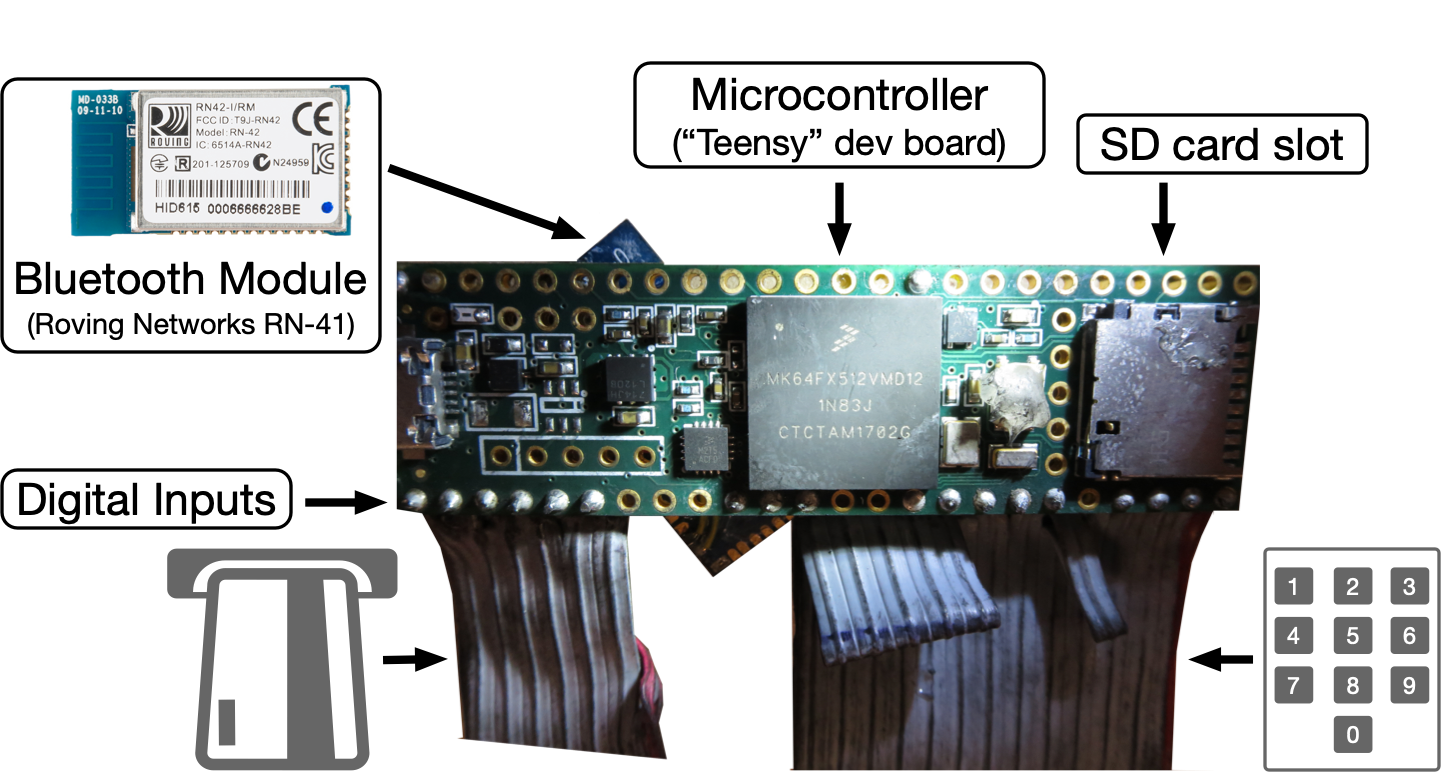
\includegraphics[width=0.95\linewidth]{fig/teensy_skimmer}
\caption{
\label{fig:intskimmer-construction}
An Internal skimmer constructed with commodity hardware. This skimmer
was detected with \bluetana in a fuel dispenser in San Juan Capistrano, CA.
}
\end{figure}

Figure~\ref{fig:intskimmer-construction} shows the components of such a
skimmer, and how they connect to the existing PoS terminal.
%
Internal skimmers read card information and PIN numbers by directly tapping into
the digital signals coming from the card reader and the PIN keypad.
%
The following is a description of the primary components of internal skimmers:
 
\paragraph{Card reader interceptor:}
%
The card reader contains an IC that converts the analog magnetic track signal encoded in ``Frequency
/ Double Frequency (F2F)'' format (ISO/IEC 7811) into a digital serial signal which is
then transmitted over a ribbon cable. The skimmer taps into this ribbon cable to intercept the credit card data.

\paragraph{PIN keypad interceptor:}
%
The PIN keypad on many PoS terminals is a digital button matrix 
connected by a ribbon cable to the Point-of-Sale circuit.
%
The signal is read
by the GPIO pins on the skimmer's microcontroller.

\paragraph{Storage:}
%
The microcontroller buffers all skimmed card information in persistent storage
(e.g., flash) until the criminal returns to wirelessly exfiltrate the captured
data, at which point the buffer is cleared so law enforcement does not know
what card numbers the criminals have.
%
One of the common storage devices discovered in prior skimmers is a
10~Mbit EEPROM chip that can hold thousands of card numbers.

\paragraph{Wireless exfiltration:}
%
The microcontroller is connected to an off-the-shelf Bluetooth module.
%
This allows the criminal to remotely exfiltrate the card information stored on
the internal skimmer's persistent storage from the comfort of their car.
%
The advantage of using commodity Bluetooth modules is that they are
interoperable with almost all computing devices---criminals do not look
suspicious if they are caught with exfiltration tools.
%
Bluetooth also makes it possible for criminals to hire this job out to associates without special skills.

\paragraph{Power:}
%
The card reader needs DC power (generally 5V) to power its F2F decoder IC.
%
Internal skimmers already tap into these cables to collect card numbers.
Conveniently, they also get power without any additional effort.

\subsubsection{Creating skimmers with commodity hardware}
\label{sec:background:commodity}
%
There are many implementations of internal skimmers in use today.
%
Some are custom circuits, but many are made by cobbling together several
commodity devices (e.g., the Teensy dev board and RN-41 shown in
Figure~\ref{fig:intskimmer-construction}).
%
The most common example of this are the internal skimmers made by modifying
commercial handheld card skimmer circuits (e.g., Deftun MiniDX3):
%
handheld skimmers used by criminals to to ``double swipe'' a
card~\cite{cardforensics} and store data for later retrieval from a PC.
%
These devices can be modified to operate as fuel dispenser skimmers by: (1)
disconnecting the skimmer's own card reader, and soldering wires from the gas
pumps's reader, (2) attaching a commercial Bluetooth module by soldering it to
the serial I/O pins on the skimmer's microcontroller, (3) wiring the power from
the dispenser's card reader to power the skimmer.
%}}}

\subsection{Internal skimmers are easy to install} %{{{
\label{sec:background:install}

\begin{figure}
\centering
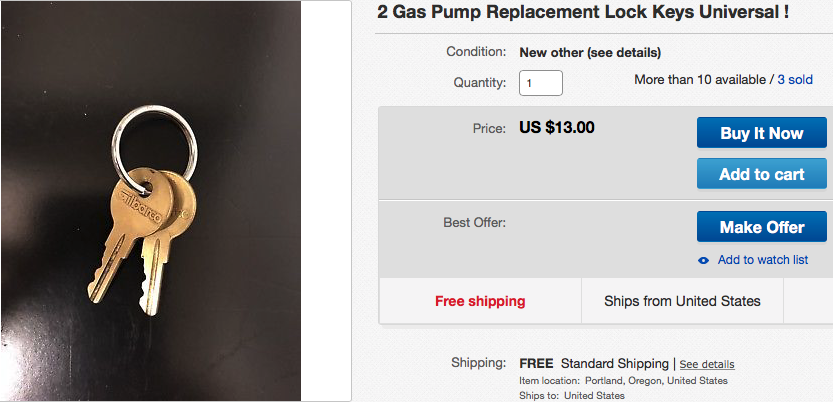
\includegraphics[width=\linewidth]{fig/universalkey.png}\\
\caption{
\label{fig:universalkey}
Criminals can buy keys for dispensers online.
}
\end{figure}

Several fuel dispensers installed in the early 2000s have poor physical security
for the payment circuitry.
%
Some fuel dispensers can be accessed without keys (e.g., Wayne Ovation): the
criminal simply has to remove a few screws to open the door.
%
Others require a universal key to open the door (e.g., Gilbarco Advantage): the
criminal simply has to purchase one of these keys online to open the door (e.g.,
the eBay listing shown in Figure~\ref{fig:universalkey}).
  
Fuel stations are slowly upgrading to newer dispensers that have better
physical security.
%
However, dispenser upgrades are a costly undertaking for the approximately 150,000 fuel
stations in the US~\cite{npn-station-count}, the vast majority of which are
independently owned and operated.
%
Furthermore, upgrade pumps to EMV chip cards has been delayed by three
years due to lack of compliance~\cite{emv2020}. \noteby{MB}{We mention this elsewhere. Should we bother mentioning it again?}
%
It is an open area of research to develop physical security measures that can
also accommodate regular access by authorized parties, some proposals include
costly per-dispenser door alarms, and complicated keying
systems~\cite{instakey}.

\begin{figure}
\centering
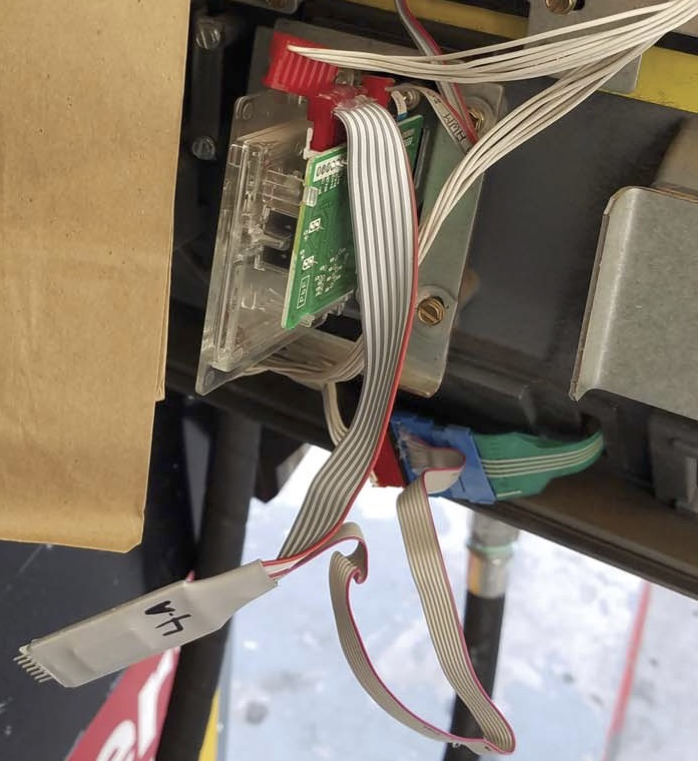
\includegraphics[width=0.8\linewidth]{fig/intskimmer-installation}\\
\small{(Photo from Arizona Department of Weights and Measures)}
\caption{
\label{fig:intskimmer-installation}
An internal skimmer taps into the payment cabling inside the enclosure of a
  compromised fuel dispenser detected by \bluetana in Tempe, AZ.
}
\end{figure}

% Next we describe how a criminal can easily and quickly attach internal skimmer
% to a fuel dispenser's payment system.
% \noteby{MB}{Oof, take this out and reformat the section below this point;
% this comes out of nowhere and lasts for a total of two paragraphs. Integrate
% this in}
% %
% Fuel dispensers are the most prominent target for internal skimmers\footnote{
% Internal skimmers have also been discovered in train station ticketing
% machines and retail PoS terminals.}
% %
% All internal skimmers capture payment information from the magnetic card
% reader\footnote{We discuss internal skimmers for EMV chip cards in
% Section~\ref{sec:discussion:emv}.}, some also capture PINs from the keypad.

If accessing a pump's internals is trivial, so is attaching a skimmer.
%
The attacker taps into the ribbon cables that attach the magnetic stripe reader
(and optionally the pinpad) to the main PoS circuit.
%
Commonly, this is done either by tapping a secondary header into the cable, or
adding a new pass-through cable (this was the method used on the dispenser shown
in Figure~\ref{fig:intskimmer-installation}).
%
The internal skimmer circuit board itself is hidden inside a pre-added
rubberized material (e.g., heat-shrink tubing or electrical tape) to match the
reset of the internal wiring.

In order to evaluate the current state of pump security, we estimated the
proportion of pumps that are vulnerable to universal key attacks by surveying
fuel dispenser deployments. \noteby{MB}{We've also done this for a random
sampling of pumps across the country. We should also make the transition into
this point from the prior paragraph smoother}
%
Specifically, we used Google Street View to manually classify the fuel dispenser
make/model of the 875 gas stations in in one of the ten largest cities in the
United States.
%
We found that 31\% (271) of the stations were using a popular model of
dispenser that has a universal key.
% 
We found that the vulnerable dispensers are installed in both the urban and
suburban areas, although the concentration is in rural areas. \noteby{MB}{If you say this, gimme the numbers.}
%
Although there are fewer vulnerable pumps in urban areas, these locations are
still targeted: we discovered one urban gas station compromised by skimmers on
seven dispensers---all but one in the station.

%}}}

% Extra text {{{
\if 0

Credit card theft at point-of-sale terminals has been a menacing occurence for
many years, with gas stations and ATMs being common targets. Consequently, due
to this construction, we can group credit card theft devices (hereafter
referred to as skimmers) under two groups, based on the possible opportunities
to attach a skimmer: 

\begin{enumerate}
	\item \textbf{External skimmers :} External skimmers are generally planted on the outer read head, typically in the form of an addtional read head(overlay skimmers) or as a piece of metal inserted in the read slot (shimmers). These skimmers are required to powered by a battery and contain on-board storage. These skimmers while difficult to detect right off the bat, are generally visible to the outside world. Their mode of operation is to perform a secondary read of the credit card data when the card in inserted in the slot. These are typically deployed in ATMs, and in a few cases in gas pumps as well 
	\item \textbf{Internal skimmers :} 
\end{enumerate}

Gas pumps in particular are of great interest, as the average gas pump reads
multiple cards over the normal course of its operation. 

\fi
\begin{comment}
The onboard wireless modules make data retrieval post installation very convenient for the criminals. In case of Bluetooth for instance, all that is required is to drive upto the gas station ever so often, connect to the skimmer, download the contents using a phone/tablet/laptop based app, and then leave. In most cases, the criminals even employ mules to do this job. This data collection is relatively inocuous and very difficult to identify for anyone on the scene as some criminal activity. We know this first hand, as part of our experimentation required us to drive to over 200 gas stations, and we were able to do so without raising eyebrows even once.

Amongst the myriad of wireless technologies out there, classic Bluetooth is the most popular amongst skimmer manufacturers. There a variety of reasons for that :
\begin{enumerate}
	\item There are a wide variety of commodity Bluetooth serial modules available online, for very cheap prices
	\item These modules are plug and play, and board design becomes simple and cheap
	\item Classic Bluetooth as an interface is readily available in phones/laptops/tablets for many years, and cross OS support for it is very extensive. Thus no special hardware is required for data collection efforts.
	\item While using long range wireless radios like GSM/LTE can aid remote data collection, they make forensics and criminal catching much easier. Cellular connections have a number associated with them, which adds to the cost of purchasing a cellular plan, plus increases risk as tracing of cell numbers is much easier for law enforcement. 
\end{enumerate}
\end{comment}

\begin{comment}
Card Skimmers and Shimmers (those which read from the chip
rather than the mag stipe) have been a blossoming field of
research in recent time. Previous research has been done
to detect the superficial variety of skimmers, by detecting
a double read of the mag stripe as it is used within a machine.
[1]. The forms of skimmers have advanced more rapidly than research
has alluded, however, and varieties have evolved for the purpose of
infecting potential environments.  Bluetooth and GSM enabled chips are
now readily built and deployed, as was noted in our discussions with
police and government officials in states which have high automotive
usage[2]. Bluetooth based skimmers, in particular, have become prevalent
in states such as Arizona, due to cheaply available hardware and ease
of connection with consumer electronics [3]; these skimmers, which
typically are inaccessible by physical retrieval and interface only
through wireless interfaces are referred to as ``deep-insert''.

In the gas pump environment, these skimmers are attached onto the ribbon wire
between the mag reader on the pump and the PoS system which mediates the
transaction. The device typically consists of a microcontroller, embedded
memory, and a bluetooth transciever or GSM chip. The device draws power from
the pump itself, and stores information which it intercepts as it travels
across the wire. At an undetermined point in time, a client desiring to
retrieve data from the device may connect to it via bluetooth, establish
an RFCOMM serial data transfer socket, and pull data from memory. In this
fashion, criminals are able to collect credit card data from various victims
by installing the device in a frequently-used gas pump, download it at a
later time, and then make use of this data to perform illicit purchases.

There are two downsides to such an approach: difficulty in installation 
and difficulty of retrieval. Installation requires access to the internals
of the device being skimmed itself. In the case of gas pumps, this difficulty
is variable depending upon the pump type. For older Gilbarco Brand pumps, for
instance which constituted roughly 31\% of one metropolitan area in which we
surveyed, there exists a single master key, and the ribbon wire to which the
device must be attached is accessible in the frontmost compartment accessible
by the key. Newer pumps are not as accessible, and thus require either more
expensive hardware such that a deep insert skimmer may be installed
directly via the card slot or through a time intesive process. Retrieval
requires the use of a specialized application which can interface to the
device; in the case of GSM, such an interface might be tracable if the
skimmer is discovered, and in the case of Bluetooth, someone must visit the
pump for the data to be retrieved. Bluetooth, in particular, is vulnerable to
honeypotting, a mitigation strategy which we have performed and which is
discussed in a later section.

The obvious benefit on behalf of do-gooders to a device using Bluetooth is
the existence of an interface by which the device may be discovered, however,
doing so is non-trivial, and is the focus of this paper. Detection of these
malicious devices involves hunting for abnormal signal strength patterns,
geofencing, fingerprinting of inquiry scan response data, and crowdsourced
data colleciton.

 Existing measures for securing CRIND (card reader in
dispenser) trays have been found to be lacking. Majority of gas pumps across
brands in current deployment either have straight up ejectable CRIND trays.
\end{comment}
%}}}


\begin{table}
    \centering
    \begin{tabular}{ll}
    \toprule
    \textbf{Total Tracks} & 251 \\
    \textbf{Total Tracks Recovered} & 202 \\
    \midrule
    \colname{Type} & \colname{\# of Cards}  \\
    \midrule
    \textbf{Debit} \\
    \quad with PIN & 79 \\
    \quad with ZIP & 15 \\
    \quad without P/Z & 11 \\
    \textbf{Credit} \\
    \quad with ZIP & 71 \\
    \quad with PIN & 6 \\
    \quad without P/Z & 15 \\
    \textit{Unknown BIN/IIN} & 5 \\
    \midrule
    Avg. Tracks per Skimmer & 20.2 \\
    Std. Tracks per Skimmer & TODO \\
    Value per Skimmer & TODO? \\
    Total value & TODO? \\
    \bottomrule

\end{tabular}

    \caption{Summary of skimmer track statistics from ten recovered gas station skimmers.}
    \label{tab:skim-dump-res}
\end{table}
